% =============================================================================
%  پایان‌نامه کارشناسی ارشد — دانشگاه شاهد
%  بازسازی ساختار «ShahedUniversityMScThesisTemplate.pdf» با xepersian
%
%  این پروژه فعلاً فقط فصل‌های پنجم و ششم را می‌سازد. برای تبدیل به پایان‌نامه
%  کامل، فصل‌های اول تا چهارم را در chapters/ بگذارید و \include آن‌ها را
%  (محل علامت‌گذاری‌شده) از حالت کامنت خارج کنید.
%
%  کامپایل:  xelatex main && bibtex main && xelatex main && xelatex main
%            (یا: latexmk -xelatex main.tex)
% =============================================================================
\documentclass[12pt,a4paper,oneside]{report}

\usepackage{amsmath,amssymb,amsthm}
\usepackage{graphicx}
\usepackage{booktabs}
\usepackage{array}
\usepackage{tabularx}
\usepackage{caption}
\usepackage{subcaption}
\usepackage{fancyhdr}
\usepackage{geometry}
\usepackage{setspace}
\usepackage[table]{xcolor}

\geometry{top=3.0cm,bottom=2.5cm,left=3.0cm,right=2.5cm}
\setstretch{1.5}
\captionsetup{font=small,labelfont=bf,justification=centering}

% --- فونت‌ها (روی این ماشین B Nazanin نصب است؛ در غیر این صورت عوض کنید) ------
\usepackage{xepersian}
\settextfont{B Nazanin}
\setlatintextfont{Vazirmatn}   % نسخه‌های نو xepersian؛ در نسخه‌های قدیمی‌تر: \setlatinfont
\SepMark{-}

% \num بدون بارگذاری siunitx (که در این نصب موجود نیست)
\providecommand{\num}[1]{#1}

% --- سازگاری bidi/xepersian با هسته LaTeX این نصب ---------------------------
% در این توزیع TeX Live، بسته bidi توابعی را صدا میزند که در هسته نصب وجود
% ندارند \MathCollectTrue/\MathCollectFalse و ریال@kernel@tabular@init).
% تعریف جایگزین خالی، ویژگی «تبدیل اعداد داخل جدول» را خاموش میکند ولی ساخت
% جدولهای راستبهچپ سالم میماند. اگر TeX Live را بهروز کردید، این شش خط
% را حذف کنید.
\providecommand{\MathCollectTrue}{}
\providecommand{\MathCollectFalse}{}
\makeatletter
\providecommand{\@kernel@tabular@init}{}
\makeatother

% --- قضیه‌ها و تعریف‌ها --------------------------------------------------------
\theoremstyle{definition}
\newtheorem{definition}{تعریف}[chapter]
\newtheorem{example}{مثال}[chapter]
\theoremstyle{plain}
\newtheorem{theorem}{قضیه}[chapter]
\newtheorem{lemma}{لم}[chapter]
\newtheorem{corollary}{نتیجه}[chapter]
\renewcommand{\proofname}{اثبات}

% شماره‌گذاری فارسی اعداد و «-» به‌عنوان جداکننده، پیش‌فرض xepersian است.

% =============================================================================
\begin{document}

% ------------------------------------------------------------------ صفحه عنوان
\begin{titlepage}
\centering
{\large وزارت علوم، تحقیقات و فناوری}\\[0.4cm]
{\large دانشگاه شاهد}\\[0.15cm]
{\large دانشکده علوم پایه}\\[1.2cm]

{\large پایان‌نامه برای دریافت درجه کارشناسی ارشد}\\[0.2cm]
{\large در رشته ریاضی، گرایش آنالیز عددی}\\[1.6cm]

{\Large\bfseries حل مسئله مجموعه احاطه‌گر کامل با استفاده از شبکه‌های عصبی
گرافی و یادگیری تقویتی}\\[1.8cm]

{\large نگارنده:}\\[0.15cm]
{\large محمود یوسفی}\\[1.2cm]

{\large استاد راهنما:}\\[0.15cm]
{\large جناب آقای دکتر نادر جعفری‌راد}\\[0.9cm]

{\large استاد مشاور:}\\[0.15cm]
{\large \lr{\dots\dots\dots\dots\dots\dots\dots\dots}}\\[1.2cm]

{\large ماه و سال:}\\[0.15cm]
{\large \lr{\dots\dots\dots\dots\dots\dots\dots\dots}}
\end{titlepage}

\pagenumbering{harfi}

% --------------------------------------------------------------- بسم‌الله
\thispagestyle{empty}
\vspace*{\fill}
\begin{center}
  {\Large بِسْمِ اللهِ الرَّحْمنِ الرَّحیم}
\end{center}
\vspace*{\fill}
\clearpage

% ------------------------------------------------------------ صفحه اظهارنامه
\chapter*{اظهارنامه دانشجو}
\addcontentsline{toc}{chapter}{اظهارنامه دانشجو}
اینجانب \textbf{محمود یوسفی} دانشجوی دوره کارشناسی ارشد رشته ریاضی گرایش آنالیز
عددی دانشگاه شاهد، اظهار می‌دارم که این پایان‌نامه با عنوان
«حل مسئله مجموعه احاطه‌گر کامل با استفاده از شبکه‌های عصبی گرافی و یادگیری
تقویتی» بر پایه پژوهش‌های انجام‌شده توسط اینجانب و با راهنمایی استادان
راهنما و مشاور، تهیه و تنظیم شده است، و کلیه حقوق مادی و معنوی آن متعلق به
دانشگاه شاهد است. همچنین اعلام می‌دارم که مطالب مندرج در این پایان‌نامه
حاصل کار پژوهشی خودم است و در موارد استفاده از منابع دیگران، به آن‌ها
ارجاع داده شده است.
\vspace{1.5cm}

\begin{flushleft}
  نام و نام خانوادگی: محمود یوسفی \\[0.3cm]
  تاریخ و امضا: \lr{\dots\dots\dots\dots\dots}
\end{flushleft}
\clearpage

% -------------------------------------------------------------------- تقدیم
\chapter*{تقدیم}
\addcontentsline{toc}{chapter}{تقدیم}
\vspace*{2cm}
\begin{center}
به پدر و مادرم که آموختند پرسش، آغاز دانستن است.
\end{center}
\clearpage

% -------------------------------------------------------------------- سپاسگزاری
\chapter*{سپاسگزاری}
\addcontentsline{toc}{chapter}{سپاسگزاری}
بدین‌وسیله از استاد راهنما، جناب آقای دکتر نادر جعفری‌راد، برای راهنمایی‌های
دقیق در طول انجام این پژوهش سپاسگزاری می‌کنم. همچنین از همه کسانی که در
مراحل اجرای آزمایش‌ها و بازبینی نتایج این کار یاری رساندند، قدردانی می‌کنم.
\clearpage

% -------------------------------------------------------------------- چکیده
\begin{center}
  {\Large\bfseries چکیده}
\end{center}
\vspace{0.4cm}
\noindent
مسئله مجموعه احاطه‌گر کامل یک تعمیم سخت‌گیرانه از مسئله مجموعه احاطه‌گر است که
در آن هر رأس گراف باید حداقل یک همسایه در مجموعه انتخابی داشته باشد. در این
پایان‌نامه، چارچوب یادگیری‌محور مبتنی بر شبکه عصبی گرافی و یادگیری تقویتی که
توسط \lr{Chen} و همکاران برای مسئله مجموعه احاطه‌گر ارائه شده است، بازسازی و
سپس به مسئله کامل گسترش داده می‌شود. بازسازی پویا‌سازی مسئله به‌صورت یک فرآیند
تصمیم‌گیری، محیط جدید و \lr{DDQN} انجام شد و نتایج مقاله در جدول‌های مرجع
بازتولید گردید.\
پرسش اصلی این بود که آیا اجزای همین چارچوب برای مسئله کامل قابل استفاده‌اند.
پاسخ منفی است و در قالب یک قضیه اثبات می‌شود: ماسک عمل روش مرجع هرگز جواب
شدنی برای مسئله کامل تولید نمی‌کند (این نتیجه با آزمایش روی \num{177} گراف و
یک مثال نقض کمینه روی مسیر چهاررأسی تأیید می‌شود). بنابراین فضای عمل بازطراحی
شد: انتخاب یک رأس فقط همسایه‌های آن را راضی می‌کند، حالت محیط دو کاناله
(\lr{coverage} و \lr{selection}) می‌شود و تابع پاداش از «سود پوشش» به «هزینه هر
تصمیم» تغییر می‌کند؛ دلیل این تغییر با یک قضیه نشان داده می‌شود: پاداش مقاله
در مسئله کامل بازدهی ثابت $n$ تولید می‌کند و هیچ سیگنالی برای کمینه‌سازی اندازه
ندارد.\
افزون بر این، سه بهبود ارائه و ارزیابی شد: رفع یک باگ مقیاس‌پذیری در خوانش
گراف (که باعث انفجار مقادیر ارزش بر حسب اندازه گراف می‌شد)، مجاز کردن رأس‌های
پشتیبان برگ به‌عنوان بخشی از جواب به‌جای حذف آن‌ها و دو تقویت «صفر-آموزش» شامل
پالایش خروجی و ماسک \lr{top-k} بر پایه سود. ارزیابی روی \num{168} گراف از هفت
خانواده نشان می‌دهد روش پیشنهادی از نظر آماری هم‌سطح بازارزیابی \lr{GRASP} است
ولی حدود \num{4} تا \num{25} برابر سریع‌تر جواب می‌دهد، روی لاتیس شش‌گوش به‌طور
معنادار بهتر از آن عمل می‌کند ($0.786$ در برابر $0.847$ نسبت به خط مبنای
حریصانه) و روی لاتیس و خانواده‌های اسپارس به بهینه می‌رسد. همچنین اجبار برگ‌ها
تعداد تصمیم‌های عامل را حدود \num{64}\% و زمان رسیدن به سطح نهایی را حدود
\num{3.5} برابر کاهش می‌دهد، بدون تغییر در کیفیت جواب.\

\vspace{0.5cm}
\noindent
\textbf{واژه‌های کلیدی:} مجموعه احاطه‌گر کامل، شبکه عصبی گرافی، یادگیری تقویتی،
\lr{DDQN}، بهینه‌سازی ترکیبیاتی، پوشش مجموعه‌ای، بازارزیابی \lr{GRASP}.
\clearpage

% ---------------------------------------------------------------- فهرست‌ها
\renewcommand{\contentsname}{فهرست مطالب}
\renewcommand{\listfigurename}{فهرست شکل‌ها}
\renewcommand{\listtablename}{فهرست جدول‌ها}
\tableofcontents
\clearpage
\listoffigures
\clearpage
\listoftables
\clearpage

\pagenumbering{arabic}

% =============================================================================
% فصل‌ها
%   فصل‌های اول تا چهارم در فایل Word نوشته شده‌اند؛ پس از انتقال آن‌ها به
%   همین قالب، خطوط زیر را از حالت کامنت خارج کنید.
\chapter{مقدمه}
\label{ch:intro}

\section{مقدمه کلی}

گراف‌ها ابزاری قدرتمند برای مدلسازی روابط بین موجودیت‌ها در بسیاری از سیستم‌های واقعی هستند. از شبکه‌های اجتماعی و زیستی گرفته تا شبکه‌های مخابراتی، حمل‌ونقل و حسگر بی‌سیم، ساختار گرافی نقش کلیدی در تحلیل و درک این سیستم‌ها ایفا می‌کند \cite{alanko2010}.

با افزایش اندازه و پیچیدگی گراف‌های دنیای واقعی، روش‌های سنتی تحلیل داده‌ها دیگر پاسخگوی این حجم از اطلاعات نیستند و نیاز به الگوریتم‌های تخصصی گراف بیش از پیش احساس می‌شود. این الگوریتم‌ها با بهره‌گیری از ویژگی‌های ساختاری گراف، امکان تحلیل، بهینه‌سازی و تصمیم‌گیری مؤثر را فراهم می‌کنند \cite{bengio2021, bondy2008}.

\section{مسائل بهینه‌سازی روی گراف}

در بسیاری از کاربردهای عملی، هدف صرفاً تحلیل ساختار گراف نیست، بلکه یافتن راه‌حل‌های بهینه برای مسائل تعریف‌شده بر روی آن اهمیت ویژه‌ای دارد. مسائل بهینه‌سازی گراف به یکی از شاخه‌های بنیادی علوم کامپیوتر، تحقیق در عملیات و هوش مصنوعی تبدیل شده‌اند. در این مسائل، هدف معمولاً انتخاب یا سازمان‌دهی مجموعه‌ای از رأس‌ها یا یال‌ها به‌گونه‌ای است که ضمن رعایت مجموعه‌ای از محدودیت‌ها، یک معیار مشخص بهینه شود \cite{paschos2010}.

از جمله مسائل شناخته‌شده در این حوزه می‌توان به کوتاه‌ترین مسیر، درخت پوشای کمینه، رنگ‌آمیزی گراف، پوشش رأس، خوشه‌بندی و مجموعه مستقل اشاره کرد. این مسائل در کاربردهای متنوعی نظیر طراحی شبکه‌های ارتباطی، زمان‌بندی، تخصیص منابع، مسیریابی، امنیت شبکه و تحلیل سیستم‌های پیچیده به‌کار می‌روند.

در میان این مسائل، مسئله مجموعه احاطه‌گر\footnote{Dominating Set} به‌دلیل کاربردهای گسترده و پیچیدگی محاسباتی بالا، جایگاه ویژه‌ای دارد. این مسئله در حوزه‌هایی مانند طراحی شبکه‌های حسگر بی‌سیم، مکان‌یابی تسهیلات، پایش شبکه‌های ارتباطی، کنترل و نظارت بر زیرساخت‌ها و بسیاری از سیستم‌های توزیع‌شده کاربرد فراوانی دارد \cite{haynes1998fundamentals, ore1962theory}.

\section{معرفی مسئله مجموعه احاطه‌گر}

مسئله مجموعه احاطه‌گر ($DS$) یکی از مسائل پایه‌ای نظریه گراف است. فرض کنید $G=(V,E)$ یک گراف ساده و متناهی باشد. مجموعه $D \subseteq V$ را یک مجموعه احاطه‌گر می‌نامیم هرگاه هر رأس $v \in V$ یا عضوی از $D$ باشد یا حداقل با یکی از رأس‌های موجود در $D$ مجاور باشد \cite{haynes1998fundamentals}.

هدف مسئله مجموعه احاطه‌گر کمینه، یافتن کوچک‌ترین مجموعه احاطه‌گر از نظر تعداد اعضا در گراف داده‌شده است. این مسئله برای حالت کلی NP-کامل است \cite{garey1979computers}.

\section{مسئله مجموعه احاطه‌گر کامل}

یکی از تعمیم‌های مهم مسئله مجموعه احاطه‌گر، مسئله مجموعه احاطه‌گر کامل\footnote{Total Dominating Set} ($TDS$) است. در این نسخه، شرط سخت‌گیرانه‌تر این است که هر رأس باید حداقل یک همسایه در مجموعه انتخاب‌شده داشته باشد؛ به‌بیان دیگر، هیچ رأسی نباید تنها توسط خودش احاطه شود و همچنین رأس‌های داخل مجموعه نیز باید توسط رأس دیگری از مجموعه احاطه گردند \cite{haynes1998fundamentals}.

فرموله‌سازی دقیق‌تر این مسئله در فصل \ref{ch:tdsp-extension} آمده است. مسئله مجموعه احاطه‌گر کامل نیز NP-کامل بوده و در بسیاری از کاربردهای عملی نظیر شبکه‌های حسگر بی‌سیم، کنترل ترافیک و سیستم‌های نظارتی اهمیت دارد.

\section{انگیزه پژوهش}

روش‌های دقیق برای حل مسائل NP-کامل تنها برای گراف‌های کوچک کارآمدند. با بزرگ شدن اندازه گراف‌ها، نیاز به روش‌های تقریبی و هوشمند افزایش می‌یابد. در سال‌های اخیر، ترکیب یادگیری عمیق با یادگیری تقویتی و شبکه‌های عصبی گرافی\footnote{Graph Neural Networks} توانسته است نتایج امیدوارکننده‌ای در حل مسائل ترکیبیاتی روی گراف ارائه دهد \cite{gilmer2017mpnn, khalil2017learning, bello2016neural}.

مقاله \cite{chen2024dsp} رویکردی مبتنی بر شبکه عصبی گرافی و یادگیری تقویتی دوگانه ($DDQN$) را برای مسئله مجموعه احاطه‌گر ارائه داده است. این پژوهش با هدف بررسی امکان‌پذیری گسترش همین چارچوب به مسئله مجموعه احاطه‌گر کامل و بهبود عملکرد آن انجام شده است.

\section{ساختار پایان‌نامه}

این پایان‌نامه در شش فصل تنظیم شده است. در فصل \ref{ch:theory} مبانی نظری لازم شامل نظریه گراف، یادگیری تقویتی و شبکه‌های عصبی گرافی بیان می‌شود. فصل \ref{ch:literature} به مرور پیشینه پژوهش می‌پردازد. فصل \ref{ch:reference} به بازسازی و پیاده‌سازی روش مرجع می‌پردازد. فصل \ref{ch:tdsp-extension} گسترش روش به مسئله مجموعه احاطه‌گر کامل و تحلیل نتایج را ارائه می‌دهد. فصل \ref{ch:conclusion} نیز شامل جمع‌بندی، دستاوردها، محدودیت‌ها و پیشنهادهای آینده است.

\chapter{مبانی نظری}
\label{ch:theory}

\section{مقدمه}

در این فصل، مفاهیم بنیادی موردنیاز برای درک مسئله مجموعه احاطه‌گر، شبکه‌های عصبی گرافی و یادگیری تقویتی بیان می‌شود. ابتدا مفاهیم نظریه گراف مرور شده، سپس یادگیری تقویتی و در نهایت شبکه‌های عصبی گرافی معرفی می‌گردد.

\section{مبانی نظریه گراف}

نظریه گراف شاخۀ مهمی از ریاضیات گسسته است که برای مدلسازی روابط بین اشیاء به‌کار می‌رود. یک گراف ساده $G=(V,E)$ متشکل از مجموعه‌ای متناهی از رأس‌ها $V$ و مجموعه‌ای از یال‌ها $E \subseteq \{\{u,v\} \mid u,v \in V, u \neq v\}$ است \cite{bondy2008}.

\subsection{تعاریف پایه}

\begin{definition}[همسایگی]
مجموعه همسایگان رأس $v$ که با $N(v)$ نشان داده می‌شود، شامل تمام رأس‌های مجاور با $v$ است. همسایگی بسته $N[v]=N(v)\cup\{v\}$ تعریف می‌شود \cite{bondy2008}.
\end{definition}

\begin{definition}[درجه رأس]
درجه رأس $v$ برابر با $|N(v)|$ و با $deg(v)$ نمایش داده می‌شود \cite{bondy2008}.
\end{definition}

\subsection{مجموعه احاطه‌گر و مجموعه احاطه‌گر کامل}

\begin{definition}[مجموعه احاطه‌گر]
مجموعه $D \subseteq V$ یک مجموعه احاطه‌گر است اگر برای هر $v \notin D$، حداقل یک $u \in D$ وجود داشته باشد به‌طوری‌که $\{u,v\} \in E$؛ یعنی $\bigcup_{u\in D} N[u] = V$ \cite{haynes1998fundamentals}.
\end{definition}

\begin{definition}[مجموعه احاطه‌گر کامل]
مجموعه $T \subseteq V$ یک مجموعه احاطه‌گر کامل است اگر هر رأس $v \in V$ حداقل یک همسایه در $T$ داشته باشد؛ یعنی $\bigcup_{u\in T} N(u)=V$ \cite{haynes1998fundamentals}.
\end{definition}

تفاوت اساسی این است که در مجموعه احاطه‌گر کامل، رأس‌های عضو $T$ نیز باید توسط رأس دیگری از $T$ احاطه شوند؛ بنابراین هیچ رأس تنهای در $T$ نمی‌تواند نیاز همسایه‌اش را برطرف کند. این شرط، مسئله را برای کاربردهایی که نیاز به پوشش دوطرفه یا نظارت متقابل دارند، مناسب‌تر می‌سازد.

\section{یادگیری تقویتی}

یادگیری تقویتی\footnote{Reinforcement Learning (RL)} شاخه‌ای از یادگیری ماشین است که در آن یک عامل\footnote{Agent} از طریق تعامل با محیط\footnote{Environment} یاد می‌گیرد تا تصمیم‌گیری بهینه انجام دهد. در هر گام $t$، عامل حالت $s_t$ را مشاهده کرده، عمل $a_t$ را انتخاب می‌کند و پاداش $r_t$ دریافت می‌نماید \cite{sutton2018reinforcement}.

فرآیند تصمیم‌گیری مارکوف\footnote{Markov Decision Process (MDP)} معمولاً با پنج‌تایی $(S,A,P,R,\gamma)$ مدلسازی می‌شود. تابع ارزش $Q(s,a)$ مقدار مورد انتظار پاداش تجمعی آینده را پس از انتخاب عمل $a$ در حالت $s$ نشان می‌دهد.

\subsection{یادگیری Q عمیق دوگانه}

الگوریتم $DQN$ با استفاده از شبکه عصبی برای تقریب تابع $Q$ معرفی شد \cite{mnih2015human}. اما $DQN$ دچار بیش‌برآورد\footnote{Overestimation} مقادیر $Q$ می‌شود. برای رفع این مشکل، روش $Double\ DQN$\footnote{DDQN} پیشنهاد گردید که عمل انتخاب و ارزیابی ارزش را بین دو شبکه جداگانه تقسیم می‌کند \cite{vanhasselt2016ddqn}.

در $DDQN$، عمل با استفاده از شبکه آنلاین انتخاب و ارزش آن با شبکه هدف ارزیابی می‌شود:
$$
y_t = r_t + \gamma\, Q_{\theta^-}(s_{t+1}, \arg\max_a Q_\theta(s_{t+1},a))
$$
که $\theta$ پارامترهای شبکه آنلاین و $\theta^-$ پارامترهای شبکه هدف هستند.

\section{شبکه‌های عصبی گرافی}

شبکه‌های عصبی گرافی\footnote{Graph Neural Networks (GNNs)} خانواده‌ای از مدل‌های یادگیری عمیق هستند که مستقیماً روی داده‌های گرافی عمل می‌کنند. برخلاف شبکه‌های متعارف، GNNها قادرند ساختار توپولوژیکی گراف و اطلاعات رأس‌ها را به‌طور همزمان در نظر بگیرند \cite{scarselli2008graph, gilmer2017mpnn}.

\subsection{شبکه عصبی پیام‌رسان}

معماری رایج در GNNها، شبکه عصبی پیام‌رسان\footnote{Message Passing Neural Network (MPNN)} است. در هر لایه، هر رأس پیام‌هایی را از همسایگانش جمع‌آوری، آن‌ها را ترکیب و نمایش جدید خود را به‌روزرسانی می‌کند \cite{gilmer2017mpnn}.

فرآیند پیام‌رسانی به‌صورت زیر انجام می‌شود:
$$
m_v^{(k+1)} = \sum_{u \in N(v)} M_k(h_v^{(k)}, h_u^{(k)}, e_{vu})
$$
$$
h_v^{(k+1)} = U_k(h_v^{(k)}, m_v^{(k+1)})
$$
که $h_v^{(k)}$ نمایش رأس $v$ در لایه $k$، $M_k$ تابع پیام و $U_k$ تابع به‌روزرسانی است.

\section{خلاصه}

در این فصل مفاهیم پایه نظریه گراف، مسئله مجموعه احاطه‌گر و کامل، یادگیری تقویتی و شبکه‌های عصبی گرافی مرور شد. این مبانی، زیربنای روش پیشنهادی در فصل‌های بعدی را تشکیل می‌دهند.

\chapter{مرور پیشینه پژوهش}
\label{ch:literature}

\section{مقدمه}

در این فصل، پژوهش‌های مرتبط با حل مسائل ترکیبیاتی با استفاده از یادگیری تقویتی، شبکه‌های عصبی گرافی و همچنین روش‌های موجود برای مسئله مجموعه احاطه‌گر و مجموعه احاطه‌گر کامل مرور می‌شوند.

\section{حل مسائل ترکیبیاتی با یادگیری تقویتی و شبکه‌های عصبی گرافی}

استفاده از یادگیری عمیق برای حل مسائل بهینه‌سازی ترکیبیاتی در سال‌های اخیر مورد توجه زیادی قرار گرفته است. خلیل و همکاران \cite{khalil2017learning} رویکردی مبتنی بر $DQN$ و $GNN$ برای حل مسائل NP-سخت مانند مجموعه مستقل بیشینه، حداقل پوشش رأسی و فروشنده دوره‌گرد ارائه دادند.

بللو و همکاران \cite{bello2016neural} با استفاده از یادگیری تقویتی و رمزگذار-رمزگشا\footnote{Encoder-Decoder}، روشی برای بهبود راه‌حل‌های مسئله فروشنده دوره‌گرد معرفی کردند. وینیالز و همکاران \cite{vinyals2015pointer} نیز مدل $Pointer\ Network$ را برای تولید دنباله‌های مرتب‌شده در مسائل ترکیبیاتی پیشنهاد دادند.

همچنین بنگیو و همکاران \cite{bengio2021} مروری جامع بر کاربرد یادگیری ماشین در بهینه‌سازی ترکیبیاتی ارائه نمودند و نشان دادند که روش‌های یادگیری‌محور می‌توانند در مواردی از روش‌های سنتی پیشی بگیرند یا مکمل آن‌ها باشند.

\section{پژوهش‌های مرتبط با مسئله مجموعه احاطه‌گر}

مسئله مجموعه احاطه‌گر از دیرباز مورد توجه پژوهشگران بوده است. روش‌های حریصانه، الگوریتم‌های تقریبی و فراابتکاری متعددی برای این مسئله ارائه شده‌اند \cite{haynes1998fundamentals}.

در سال‌های اخیر، رویکردهای یادگیری‌محور نیز ظهور کرده‌اند. چن و همکاران \cite{chen2024dsp} اولین بار چارچوبی یکپارچه مبتنی بر شبکه عصبی گرافی و $DDQN$ را برای حل مسئله مجموعه احاطه‌گر ارائه دادند. در این روش، مسئله به‌صورت فرآیند تصمیم‌گیری ترتیبی مدلسازی شده و عامل یاد می‌گیرد با انتخاب رأس‌های مناسب، مجموعه احاطه‌گر با اندازه کوچک تولید کند.

این روش در مقایسه با الگوریتم‌های حریصانه و برخی روش‌های فراابتکاری، نتایج قابل‌قبولی روی خانواده‌های مختلف گراف از جمله گراف‌های تصادفی $ER$، درخت‌ها و شبکه‌های واقعی نشان داده است.

\section{پژوهش‌های مرتبط با مسئله مجموعه احاطه‌گر کامل}

مسئله مجموعه احاطه‌گر کامل نیز موضوع پژوهش‌های فراوانی بوده است. تحقیقات زیادی بر روی کران‌های بالا و پایین، پیچیدگی محاسباتی و الگوریتم‌های تقریبی این مسئله متمرکز بوده‌اند \cite{haynes1998fundamentals, cockayne2004total}. با این حال، تاکنون تلاش محدودی برای حل این مسئله با استفاده از یادگیری تقویتی و شبکه‌های عصبی گرافی انجام شده است.

با توجه به شباهت ساختاری بین مسئله مجموعه احاطه‌گر و مجموعه احاطه‌گر کامل، طبیعی است که بررسی شود آیا چارچوب پیشنهادی در \cite{chen2024dsp} قابل گسترش به نسخه کامل این مسئله باشد یا خیر. این پرسش، انگیزه اصلی پژوهش حاضر را تشکیل می‌دهد.

\section{خلاصه}

در این فصل، پیشینه پژوهش در سه حوزه مرور شد: حل مسائل ترکیبیاتی با RL و GNN، روش‌های موجود برای مسئله مجموعه احاطه‌گر و روش‌های مرتبط با مجموعه احاطه‌گر کامل. بررسی‌ها نشان می‌دهد که اگرچه روش‌های یادگیری‌محور برای DSP موفق بوده‌اند، گسترش مستقیم آن‌ها به TDSP نیازمند بازنگری در فضای عمل، حالت و تابع پاداش است که در فصل \ref{ch:tdsp-extension} به آن پرداخته می‌شود.

\chapter{بازسازی و پیاده‌سازی روش مرجع}
\label{ch:reference}

\section{مقدمه}

در این فصل، روش مرجع ارائه‌شده در \cite{chen2024dsp} برای حل مسئله مجموعه احاطه‌گر با استفاده از شبکه عصبی گرافی و یادگیری تقویتی دوگانه بازسازی و پیاده‌سازی می‌شود. هدف، اطمینان از درک صحیح چارچوب و ایجاد پایه‌ای برای گسترش آن به مسئله مجموعه احاطه‌گر کامل است.

\section{مدلسازی مسئله به‌صورت فرآیند تصمیم‌گیری مارکوف}

روش مرجع، مسئله مجموعه احاطه‌گر را به‌صورت یک فرآیند تصمیم‌گیری ترتیبی مدلسازی می‌کند. در هر گام، عامل یکی از رأس‌های مجاز را انتخاب می‌کند تا به مجموعه $S$ افزوده شود. حالت محیط با بردار ویژگی هر رأس و ساختار گراف توصیف می‌شود \cite{chen2024dsp}.

\section{معماری شبکه عصبی گرافی}

شبکه عصبی به‌کاررفته در این روش از نوع MPNN است. نمایش اولیه هر رأس با بردار ویژگی‌ای شامل اطلاعاتی نظیر درجه رأس و وضعیت پوشش آن ساخته می‌شود. سپس با عبور از چند لایه پیام‌رسانی، نمایش‌های غنی‌تری تولید شده و در نهایت برای پیش‌بینی مقادیر $Q$ هر عمل مجاز به‌کار می‌روند \cite{gilmer2017mpnn, chen2024dsp}.

\section{الگوریتم یادگیری تقویتی دوگانه}

برای آموزش عامل از الگوریتم $Double\ DQN$ استفاده می‌شود. حافظه تجربه\footnote{Replay Buffer} برای ذخیره انتقال‌ها و نمونه‌برداری تصادفی جهت شکستن همبستگی، به‌کار می‌رود. همچنین هدف‌گیری آرام\footnote{Soft Target Update} برای افزایش پایداری یادگیری اعمال می‌گردد \cite{vanhasselt2016ddqn, mnih2015human}.

\section{طراحی فضای عمل و ماسک عمل}

در روش مرجع، در هر حالت تنها رأس‌های «مجاز» می‌توانند انتخاب شوند. این محدودسازی باعث کاهش فضای جستجو و تسریع یادگیری می‌گردد. انتخاب رأس‌های نامجاز طبق قواعد تعریف‌شده در محیط، از طریق ماسک عمل\footnote{Action Masking} غیرفعال می‌شود \cite{chen2024dsp}.

\section{پیاده‌سازی و بازتولید نتایج}

با پیاده‌سازی دقیق چارچوب فوق، تلاش شد نتایج گزارش‌شده در \cite{chen2024dsp} روی خانواده‌های گراف استاندارد بازتولید گردد. این بازتولید، پایه لازم برای تحلیل صحت پیاده‌سازی و مقایسه بعدی با نسخه گسترش‌یافته به مسئله مجموعه احاطه‌گر کامل را فراهم می‌کند.

\section{خلاصه}

در این فصل، روش مرجع مبتنی بر $GNN + DDQN$ برای مسئله مجموعه احاطه‌گر بازسازی شد. مفاهیم کلیدی شامل مدلسازی ترتیبی، MPNN، $DDQN$، حافظه تجربه و ماسک عمل بیان گردید. این پیاده‌سازی، نقطه شروع گسترش به مسئله مجموعه احاطه‌گر کامل در فصل بعدی خواهد بود.

% =============================================================================
%  فصل پنجم — گسترش چارچوب به مسئله مجموعه احاطه‌گر کامل
%  همه اعداد این فصل از خروجی‌های ذخیره‌شده در results/tdsp بازخوانی شده‌اند.
%  مولد جدول‌ها و شکل‌ها: experiments/tdsp/ch5_report.py و ch5_example.py
% =============================================================================
\chapter{گسترش چارچوب به مسئله مجموعه احاطه‌گر کامل}
\label{ch:tdsp}

\section{مقدمه و صورت مسئله}
\label{sec:tdsp-intro}

فصل چهارم چارچوب مرجع \lr{Chen} و همکاران را بازسازی کرد؛ در آن چارچوب، مسئله
\emph{مجموعه احاطه‌گر} (\lr{DSP}) حل می‌شود: زیرمجموعه‌ای از رأس‌ها انتخاب می‌شود
که هر رأس گراف یا خود در آن مجموعه باشد یا حداقل یک همسایه در آن داشته باشد.
پرسش این فصل، نسخه سخت‌گیرانه‌تر همان مسئله است.

\begin{definition}[مجموعه احاطه‌گر کامل]
\label{def:tds}
برای گراف بدون جهت $G=(V,E)$، مجموعه $S\subseteq V$ یک \emph{مجموعه احاطه‌گر کامل}
(\lr{TDS}) است اگر هر رأس $v\in V$ حداقل یک همسایه در $S$ داشته باشد:
\begin{equation}
\forall v \in V:\quad N(v)\cap S \neq \emptyset .
\label{eq:tds-def}
\end{equation}
عدد احاطه‌گری کامل $\gamma_t(G)$ کمینه اندازه چنین مجموعه‌ای است.
\end{definition}

تفاوت با \lr{DSP} در یک واژه است: در \lr{DSP} رأس می‌تواند «خودش» نیاز را برآورده
کند، اما در \lr{TDSP} باید \emph{همسایه‌ای درون مجموعه} داشته باشد. سه پیامد
فوری این تفاوت:

\begin{enumerate}
  \item هیچ رأس منزوی نمی‌تواند در جوابی معتبر حضور داشته باشد؛ بنابراین گراف باید
        درجه کمینه حداقل یک داشته باشد و در محاسبات این فصل گراف‌های دارای رأس منزوی
        کنار گذاشته می‌شوند.
  \item هر عضو $S$ باید «پشتیبان» داشته باشد: رأسی که آن را احاطه کند. پس خروجی
        نمی‌تواند مجموعه‌ای مستقل باشد.
  \item شرط پایان فرآیند تصمیم‌گیری عوض می‌شود: در \lr{DSP} پایان یعنی «همه رأس‌ها
        پوشش داده شده‌اند»؛ در \lr{TDSP} یعنی «همه رأس‌ها همسایه‌ای در $S$ دارند»،
        و این دو نه‌فقط متفاوت، بلکه برای رأس‌های عضو مجموعه ناسازگارند.
\end{enumerate}

هر دو مسئله \lr{NP}-سخت‌اند و در ادبیات، \lr{TDSP} معادل دقیق یک مسئله
\emph{پوشش مجموعه‌ای} است: جهان، مجموعه رأس‌هاست و برای هر رأس $u$ یک مجموعه
$N(u)$ تعریف می‌شود؛ انتخاب $u$ تمام اعضای $N(u)$ را می‌پوشاند. این مشاهده،
هم خط مبنای قوی فصل (الگوریتم \lr{GRASP}) را ممکن می‌کند و هم پالایش خروجی در
بخش~\ref{sec:boosts} را.

معیارهای ارزیابی این فصل: اندازه خروجی نسبت به بهینه $\gamma_t$ و نسبت به
خط مبنای حریصانه، نسبت به بازارزیابی (\lr{GRASP})، نرخ شدنی‌بودن، تعداد تصمیم‌های
عامل و زمان استنتاج.

\section{ساخت دومرحله‌ای و کران $2|D|$}
\label{sec:construction}

اولین پرسش طبیعی این است: آیا می‌توان \lr{TDSP} را از \lr{DSP} ساخت؟ اگر $D$ یک
مجموعه احاطه‌گر معمولی باشد، آیا می‌توان از آن یک مجموعه احاطه‌گر کامل ساخت؟

برای هر $D$ یک زیرمجموعه $A\subseteq D$ با این خاصیت انتخاب می‌کنیم که هر عضو
$D$ حداقل یک همسایه در $A$ داشته باشد (مسئله‌ای در اندازه خودِ $D$)، و
$S=A\cup (V\setminus D)$ را برمی‌گردانیم.

\begin{theorem}
\label{thm:bound}
برای هر مجموعه احاطه‌گر $D$ از گرافی بدون رأس منزوی، مجموعه $S=A\cup(V\setminus D)$
یک مجموعه احاطه‌گر کامل است و
\begin{equation}
|S| \le 2|D| .
\label{eq:bound}
\end{equation}
\end{theorem}

\begin{proof}
هر $u\in V\setminus D$ چون $D$ احاطه‌کننده است، همسایه‌ای در $D$ دارد و همان همسایه
در $S$ حضور دارد (چون $A\subseteq S$). هر $u\in D$ بنا به تعریف $A$ همسایه‌ای در
$A\subseteq S$ دارد. پس شرط \eqref{eq:tds-def} برای همه رأس‌ها برقرار است. برای
اندازه: $|S|\le |A|+|V\setminus D|\le |D|+(n-|D|)$؛ کران را نمی‌توان با این
استدلال دقیق‌تر کرد، ولی در گراف‌های چگال $|V\setminus D|$ کوچک است و کران
عملاً شل می‌ماند.
\end{proof}

شکل~\ref{fig:construction} کیفیت این ساخت را به‌ازای سه منبع برای $D$ نشان می‌دهد:
حل دقیق، حریصانه، و شبکه فصل چهارم. نتیجه‌ها دو نکته را روشن می‌کنند: نخست،
کران \eqref{eq:bound} در \emph{هیچ} نمونه‌ای نقض نشد (با \lr{assert} روی همه
گراف‌ها بررسی شد)؛ دوم، کیفیت میانی بسیار بدتر از کران است، به‌ویژه روی گراف‌های
\lr{BA} که $|D|$ بزرگ است و $D$ مستقل، خروجی را تا حدود $2.7\gamma_t$ می‌برد.
به زبان دیگر، مزیت این مسیر «تضمین» است، نه «کیفیت»؛ و همین مشاهده ما را به
بازطراحی مستقیم فضای عمل سوق داد.

\begin{figure}[ht]
  \centering
  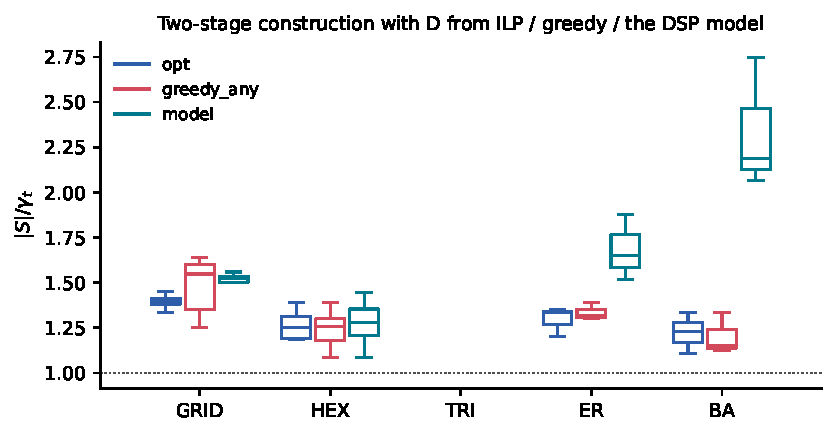
\includegraphics[width=0.85\textwidth]{figs/fig5_2_construction.pdf}
  \caption{کیفیت ساخت دومرحله‌ای ($|S|/\gamma_t$) به تفکیک خانواده گراف و منبع
  مجموعه $D$. خط‌چین، مرز بهینگی است.}
  \label{fig:construction}
\end{figure}

\section{چرا ماسک عمل مقاله برای \lr{TDSP} کار نمی‌کند؟}
\label{sec:mask}

در چارچوب مرجع، عمل مجاز فقط رأسی است که هنوز احاطه نشده باشد
($vf_v=0$)، و انتخاب $v$ خودِ $v$ و همسایه‌هایش را «احاطه‌شده» علامت می‌زند.
از این دو قاعده یک نتیجه ساختاری به‌دست می‌آید.

\begin{theorem}[ناسازگاری ماسک]
\label{thm:mask}
هر اجرای کامل سیاست مقاله (با هر قاعده انتخاب، تصادفی یا حریصانه) مجموعه‌ای
\emph{مستقل} تولید می‌کند، و بنابراین هیچ‌گاه یک مجموعه احاطه‌گر کامل نیست.
\end{theorem}

\begin{proof}
فرض کنید $u,v\in S$ و $\{u,v\}\in E$. چون $v$ با انتخاب $u$ احاطه شده است،
$vf_v=1$ می‌شود و در گام‌های بعدی $v$ از مجموعه اعمال مجاز حذف می‌شود؛ پس $v$
نمی‌تواند انتخاب شود. این با $v\in S$ در تناقض است؛ بنابراین $S$ مستقل است.
در مجموعه مستقل، هیچ عضو $S$ همسایه‌ای در $S$ ندارد، پس شرط \eqref{eq:tds-def}
برای اعضای $S$ برقرار نمی‌شود.
\end{proof}

شکل~\ref{fig:actionspace} این قضیه را تجربی تأیید می‌کند: روی \num{177} گراف از پنج
خانواده، هر سه سیاست (تصادفی، حریصانه، مدل آموزش‌دیده) خروجی مستقل دادند و
\emph{هیچ} خروجی احاطه‌گر کامل نبود. این نتیجه یک تفاوت مهم با «بدتر بودن
عملکرد» دارد: مسئله اینجا \emph{ناشدنی بودن} است، نه کیفیت پایین. پس نمی‌توان
ماسک مقاله را بدون تغییر به \lr{TDSP} منتقل کرد.

\begin{figure}[ht]
  \centering
  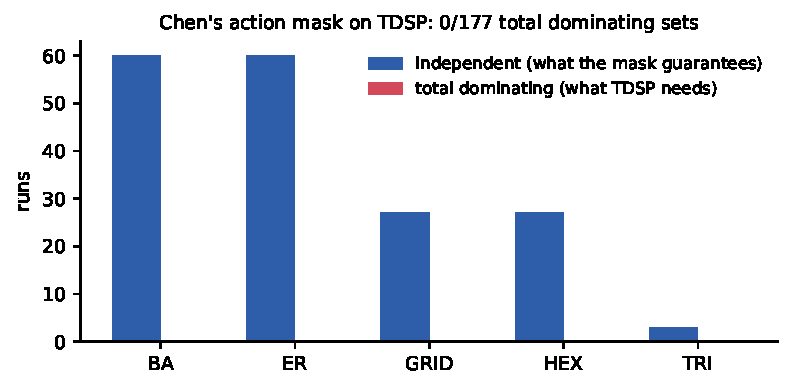
\includegraphics[width=0.8\textwidth]{figs/fig5_1_action_space.pdf}
  \caption{خروجی ماسک مقاله روی \lr{TDSP}: همه اجراها مجموعه مستقل‌اند و هیچ‌کدام
  احاطه‌کننده کامل نیست.}
  \label{fig:actionspace}
\end{figure}

کوچک‌ترین مثال نقض، مسیر $P_4$ با رأس‌های $0-1-2-3$ است. سیاست ماسک‌دار حریصانه
$S=\{1,3\}$ را می‌سازد؛ این مجموعه احاطه‌گر است و اندازه‌اش هم $2$ است، اما
رأس $3$ هیچ همسایه‌ای در $S$ ندارد، چون تنها همسایه‌اش ($2$) عضوی از مجموعه نیست.
در همین گراف، جواب بهینه مجموعاً برابر $2$ است ولی با ترکیب دیگری
($S^\ast=\{1,2\}$). شکل~\ref{fig:p4} این مغایرت را نشان می‌دهد: تفاوت در اندازه
نیست، در \emph{شدنی‌بودن} است.

\begin{figure}[ht]
  \centering
  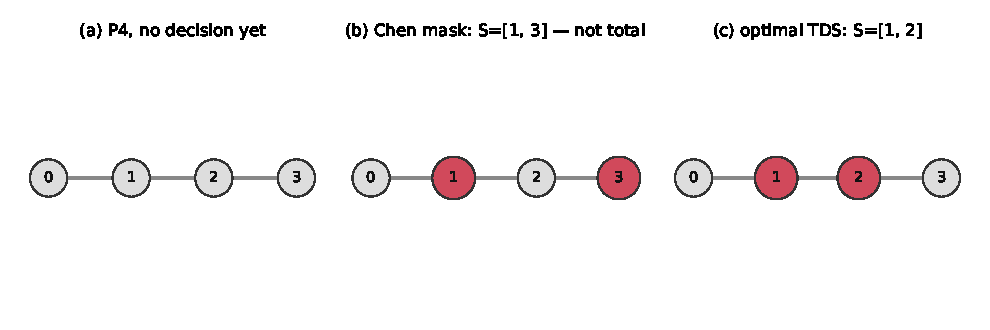
\includegraphics[width=0.92\textwidth]{figs/fig5_11_p4.pdf}
  \caption{مثال نقض روی $P_4$: (الف) گراف؛ (ب) خروجی ماسک مقاله
  ($S=\{1,3\}$) که احاطه‌گر کامل نیست؛ (ج) جواب بهینه $\{1,2\}$ با همان اندازه.}
  \label{fig:p4}
\end{figure}

\section{محیط بازطراحی‌شده: فضای عمل \lr{TDSP}}
\label{sec:env}

بر اساس بخش~\ref{sec:mask}، سه قاعده چارچوب مرجع بازنویسی می‌شود:

\begin{enumerate}
  \item \textbf{ماسک:} هر رأسی که هنوز در $S$ نیست مجاز است (نه فقط رأس‌های
        احاطه‌نشده). بنابراین اعضای $S$ می‌توانند همسایه یکدیگر باشند.
  \item \textbf{گذار:} انتخاب $v$ فقط $N(v)$ را «راضی» می‌کند و خودِ $v$ راضی
        نمی‌شود؛ پس $vf_v$ تا زمانی که همسایه‌ای انتخاب نشود صفر می‌ماند. این
        قاعده، قید احاطه‌گری کامل را به‌صورت بومی در مکانیک مسئله می‌نشاند.
  \item \textbf{پایان:} فرآیند وقتی پایان می‌یابد که همه رأس‌ها
        $vf=1$ باشند، یعنی هر رأس همسایه‌ای در $S$ داشته باشد.
\end{enumerate}

از آنجا که در مسئله جدید «عضو بودن» و «احاطه‌شده بودن» دو چیز متفاوت‌اند،
حالت محیط باید دو کانال داشته باشد:
\begin{equation}
s = \big[\,vf \;\|\; ins\,\big] \in \{0,1\}^{n\times 2},
\qquad
vf_u = \mathbb{I}\big[N(u)\cap S \neq \emptyset\big],
\qquad
ins_u = \mathbb{I}\big[u \in S\big].
\label{eq:state}
\end{equation}
اگر تنها $vf$ به شبکه داده شود، دو وضعیت متمایز (رأسی که انتخاب شده ولی هنوز
راضی نشده، و رأسی که نه انتخاب شده و نه راضی است) یکسان دیده می‌شوند و سیاست
نمی‌تواند میان آن‌ها تفکیک کند. شکل~\ref{fig:trace} (الف) و (ب) همین دو کانال را
روی یک مثال نشان می‌دهد.

نکته مهم برای بازتولید: رابط محیط ($reset/candidates/step$) عوض نشده است؛ فقط
\emph{قواعد} و \emph{ابعاد حالت} تغییر کرده‌اند. بنابراین حلقه یادگیری، شبکه
پیام‌رسان و مکانیزم \lr{DDQN} فصل چهارم بدون بازنویسی روی محیط جدید کار می‌کنند؛
تنها شرط آن است که نامزدها از خود محیط خوانده شوند (نه از $vf=0$) و شبکه
$in-ch=2$ بگیرد. سه آزمون مستقل این تطبیق را تأیید کرد: \num{118} بررسی مکانیک،
هم‌ارزی سیاست حریصانه محیط با \lr{greedy} بومی در \num{59} از \num{59} نمونه،
و بازتولید خط‌به‌خط نتایج \lr{DSP} فصل چهارم با نسخه پیشین کد (آزمون عدم رگرسیون).

\section{تابع پاداش: از «سود» به «هزینه هر تصمیم»}
\label{sec:reward}

پاداش چارچوب مرجع بر پایه تعداد رأس‌های تازه‌احاطه‌شده تعریف می‌شود. روی
\lr{TDSP} این تعریف یک اشکال ساختاری پیدا می‌کند.

\begin{theorem}
\label{thm:gain}
اگر پاداش هر گام برابر تعداد رأس‌هایی باشد که با انتخاب آن گام تازه راضی
می‌شوند (پاداش سود، یا نسخه $\pm 1$ مقاله)، بازدهی هر اپیزود مستقل از سیاست و
از اندازه مجموعه نهایی است.
\end{theorem}

\begin{proof}
شرط پایان محیط این است که همه رأس‌ها $vf=1$ شوند. هر رأس در پایان اپیزود
دقیقاً یک‌بار «تازه راضی‌شده» شمرده می‌شود؛ بنابراین مجموع سود در طول اپیزود
همیشه برابر $n$ است و بازده $n$ (یا ترکیب خطی ثابت از $n$) می‌شود، مستقل از
$|S|$.
\end{proof}

نتیجه: عاملی که این پاداش را بیشینه می‌کند هیچ انگیزه‌ای برای کوچک کردن $|S|$
ندارد؛ همه سیاست‌ها بازده یکسان می‌گیرند و سیگنال بهینه‌سازی از بین می‌رود.

\begin{definition}[پاداش هزینه]
\label{def:size-reward}
در هر تصمیم عامل پاداش $r=-1$ می‌گیرد. بنابراین بازده اپیزود برابر
$-|\text{تصمیم‌های عامل}|$ است، و اگر مجموعه اجباری $F$ (بخش~\ref{sec:forcing})
از پیش در $S$ باشد، بازده کل برابر $-|S|$ می‌شود.
\end{definition}

جدول~\ref{tab:reward} این تفاوت را روی مثال بخش~\ref{sec:example} عددگذاری می‌کند.
در سطح کل آزمایش‌ها، این تغییر ساده اثر چشمگیری داشت: میانگین
$|S|/\text{greedy}$ روی گراف‌های تصادفی بزرگ از $4.34$ به $1.04$ رسید و
مدل از «شش برابر بدتر از حریصانه» به «هم‌سطح آن» تغییر کرد؛ روی لتیس‌های
شش‌گوش، پاداش \lr{paper} کمی بهتر از پاداش هزینه بود ($0.812$ در برابر
$0.877$).

\begin{table}[ht]
  \centering
  \caption{دو تابع پاداش روی مثال گراف درختی $n=12$ (بخش~\ref{sec:example})}
  \label{tab:reward}
  \begin{tabular}{lccc}
    \toprule
    پاداش & بازده اپیزود & ارتباط با هدف & سیگنال بهینه‌سازی \\
    \midrule
    سود (نسخه مقاله) & $+12$ & مستقل از $|S|$ & ندارد \\
    هزینه ($r=-1$) & $-6$ & دقیقاً $-|S|$ & دارد \\
    \bottomrule
  \end{tabular}
\end{table}

\section{معماری شبکه: یک باگ مقیاس‌پذیری و رفع آن}
\label{sec:arch}

خوانش گراف در چارچوب مرجع، جمع نمایش رأس‌ها است: $s=\sum_{u} h_u$. این تعریف
برای $n$ ثابت بی‌ضرر است، ولی وقتی مدل فقط روی $n=20$ آموزش می‌بیند و روی
اندازه‌های دیگر آزمون می‌شود، فاجعه‌بار می‌شود: اندازه خروجی خوانش با $n$ رشد
می‌کند و مقادیر $Q$ منفجر می‌شوند. اندازه‌گیری ما: در $n=20$ مقدار $Q\approx0.8$
بود و در $n=300$ به $85183$ می‌رسید. این باگ در مسئله \lr{DSP} نیز وجود داشت
($Q\approx76379$ در $n=500$)، ولی چون مقاله برای هر اندازه یک مدل جدا آموزش
می‌دهد، در گزارش اصلی آشکار نشده است.

رفع باگ دو تغییر کوچک است: تابع تجمیع پیام‌ها از جمع به \emph{میانگین}
($\text{agg}=\text{mean}$) و خوانش گراف از $\sum h_u$ به $\frac1n\sum h_u$
($\text{mean-readout}$). پس از این تغییر، $Q$ برای همه اندازه‌ها تقریباً ثابت
می‌ماند ($\approx0.09$) و تعمیم به اندازه‌های آموزش‌ندیده ممکن می‌شود.
شکل~\ref{fig:arch} اثر این اصلاح را نشان می‌دهد: روی گراف‌های تصادفی با
$n\ge 80$ کیفیت مدل با پاداش هزینه از $4.34$ به $1.04$ بهبود می‌یابد و روی
لتیس‌ها مدل بهتر از حریصانه می‌شود ($0.81$–$0.88$).

\begin{figure}[ht]
  \centering
  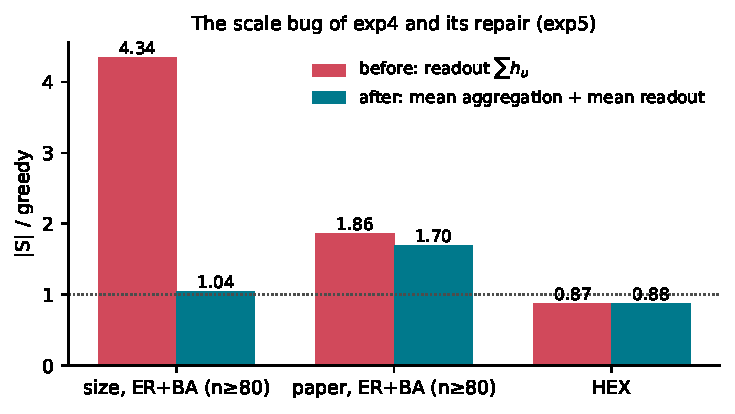
\includegraphics[width=0.72\textwidth]{figs/fig5_3_architecture.pdf}
  \caption{اثر رفع باگ مقیاس‌پذیری خوانش گراف بر کیفیت مدل.}
  \label{fig:arch}
\end{figure}

\section{دانش گراف: قواعد کاهش و اجبار برگ‌ها}
\label{sec:forcing}

نوآوری دوم پروپوزال، استفاده از مفاهیم نظریه گراف برای کاهش فضای جست‌وجو است.
سه قاعده کلاسیک بررسی شد:

\begin{enumerate}
  \item \textbf{رأس منزوی:} تنها برای تشخیص ناشدنی‌بودن مفید است.
  \item \textbf{مؤلفه‌های همبند:} تجزیه دقیق است و مسئله را به مؤلفه‌ها می‌شکند.
  \item \textbf{برگ و پشتیبان:} در \lr{DSP} معتبر است، اما در \lr{TDSP}
        \emph{نامعتبر} است.
\end{enumerate}

\begin{theorem}[نامعتبری قاعده برگ]
\label{thm:leaf-invalid}
در \lr{TDSP} نمی‌توان رأس پشتیبان یک برگ و همسایگانش را از گراف حذف کرد و
مسئله را روی گراف باقی‌مانده حل کرد.
\end{theorem}

\begin{proof}
مثال نقض: مسیر $P_3$ با رأس‌های $0-1-2$. برگ $0$ رأس $1$ را اجباری می‌کند. با
حذف $\{1\}\cup N(1)=\{0,1,2\}$ گراف خالی می‌ماند و جواب پیشنهادی $\{1\}$ است؛
اما $1$ هیچ همسایه‌ای در مجموعه ندارد و احاطه‌گری کامل برقرار نیست. جواب بهینه
$\{0,1\}$ با اندازه $2$ است. علت ساختاری: در احاطه‌گری کامل، خودِ رأس پشتیبان هم
باید پشتیبان داشته باشد، پس زیرمسئله، گراف القایی ساده نیست.
\end{proof}

پس قاعده برگ به شکل «حذف» بی‌اعتبار است. اما شکل \emph{مثبت} همان ایده معتبر است:
هر پشتیبانِ برگ در \emph{هر} جواب معتبر حاضر است، چون تنها همسایه برگ خودش است
و برگ باید توسط آن احاطه شود.

\begin{definition}[مجموعه اجباری]
\label{def:forced}
$F$ را مجموعه پشتیبان‌های برگ‌ها بگیرید. چون هر برگ درجه یک دارد، پشتیبانش در
هر مجموعه احاطه‌گر کامل حاضر است.
\end{definition}

ایده اجرایی: به‌جای حذف رأس‌ها، $F$ را در \emph{ابتدای اپیزود} در $S$ می‌نشانیم.
مکانیک $vf$ خودبه‌خود قید باقی‌مانده را حمل می‌کند: هر عضو $F$ چون خودش هم باید
پشتیبان داشته باشد، همچنان «راضی‌نشده» می‌ماند و عامل باید برایش همسایه انتخاب
کند. پاداش هزینه فقط به تصمیم‌های عامل تعلق می‌گیرد و چون $|F|$ در هر جواب
ثابت است، آفستی ثابت است و بهینه‌سازی را تغییر نمی‌دهد.

چرا این مسیر روی خانواده‌های متراکم بی‌اثر است؟ چون آن گراف‌ها برگ ندارند
($F=\emptyset$) و لتیس‌ها هم تک‌مؤلفه‌ای و بدون رأس منزوی‌اند؛ بنابراین قاعده‌های
یک و دو هم فعال نمی‌شوند. یعنی قواعد کاهش کلاسیک در این دامنه سودی ندارند — یک
نتیجه منفی که صادقانه گزارش می‌شود. اما روی خانواده‌های \emph{اسپارس} (درخت
تصادفی و \lr{BA} با $m=1$) وضعیت فرق می‌کند: پوشش $F$ تا حدود $30\%$ رأس‌ها را
می‌گیرد و صرفه‌جویی بزرگی در تعداد تصمیم ایجاد می‌کند.

جدول~\ref{tab:forcing} و شکل~\ref{fig:rlsteps} این صرفه‌جویی را نشان می‌دهند:
روی درخت‌ها، تعداد تصمیم‌های عامل برای $n=100$ از $46.6$ به $16.2$ و برای
$n=200$ از $94.3$ به $34.1$ می‌رسد (کاهش حدود $64\%$)، بدون آنکه کیفیت نهایی
تغییر کند.

\begin{table}[ht]
  \centering
  \caption{اثر اجبار برگ‌ها روی کیفیت و تعداد تصمیم (درخت تصادفی یکنواخت)}
  \label{tab:forcing}
  \begin{tabular}{lccccc}
    \toprule
    پیکربندی & $|S|/\gamma_t$ ($n=100$) & تصمیم‌ها ($n=100$) & $|S|/\gamma_t$ ($n=200$) & تصمیم‌ها ($n=200$) \\
    \midrule
    سیاست آزاد & $1.000$ & $46.6$ & $1.000$ & $94.3$ \\
    سیاست با $F$ & $1.000$ & $16.2$ & $1.000$ & $34.1$ \\
    \bottomrule
  \end{tabular}
\end{table}

\begin{figure}[ht]
  \centering
  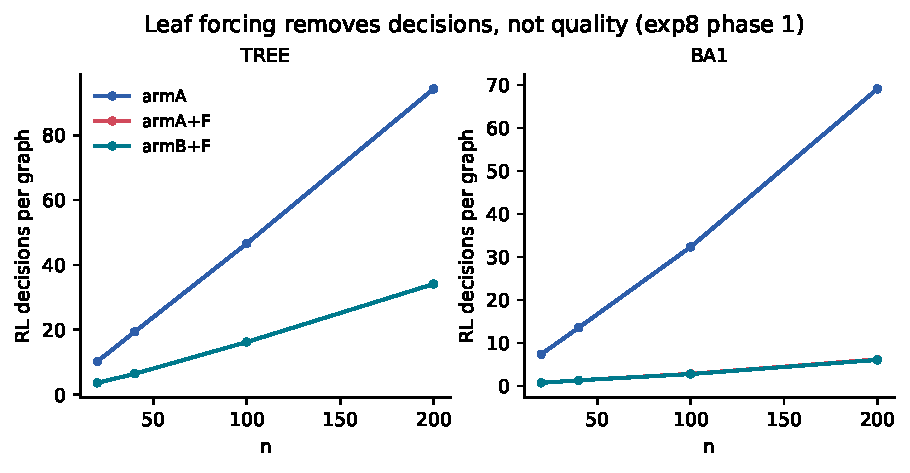
\includegraphics[width=0.85\textwidth]{figs/fig5_8_rl_steps.pdf}
  \caption{تعداد تصمیم‌های عامل به‌ازای هر گراف، با و بدون اجبار برگ‌ها.}
  \label{fig:rlsteps}
\end{figure}

اثر اجبار روی \emph{همگرایی} نیز اندازه‌گیری شد. در آزمایش زوجی با سه seed،
هر دو بازو به کیفیت نهایی یکسان رسیدند
($9.67\pm0.15$) اما بازوی دارای اجبار پس از
$43{,}333\pm10{,}408$ اپیزود به این سطح رسید و بازوی بدون اجبار پس از
$160{,}000\pm18{,}028$ اپیزود؛ یعنی \emph{حدود سه و نیم برابر} سریع‌تر. این
مقایسه زوجی است، چون با seed یکسان هر دو بازو دنباله یکسانی از گراف‌های آموزش،
مقداردهی اولیه شبکه و برنامه $\varepsilon$ می‌گیرند و تنها عامل تفاوت، خودِ اجبار
است. نکته صادقانه: مدل آموزش‌دیده با اجبار باید در زمان \emph{آزمون} هم با $F$
اجرا شود؛ اگر بدون $F$ اجرا شود، روی گراف‌های اسپارس از حریصانه بدتر عمل می‌کند.

\section{الگوریتم یادگیری: از \lr{DDQN} به سر دوگانه}
\label{sec:d3qn}

پس از تثبیت محیط، پاداش و گراف، پرسش بعدی این بود که آیا «الگوریتم یادگیری
بهتر» چیزی اضافه می‌کند؟ کوچک‌ترین تغییر ممکن، سر دوگانه
(\lr{Dueling}) است که تابع ارزش را به دو بخش تجزیه می‌کند:
\begin{equation}
Q(s,v) = V(s) + A(s,v) - \frac{1}{|\mathcal{A}(s)|}\sum_{v'\in\mathcal{A}(s)} A(s,v'),
\label{eq:dueling}
\end{equation}
که $V$ ارزش حالت و $A$ مزیت عمل است. محیط، پاداش، \lr{MPNN}، قاعده به‌روزرسانی
\lr{DDQN} و پروتکل آموزش دست‌نخورده می‌مانند و فقط سر شبکه عوض می‌شود
(فلگ \lr{--dueling}، پیش‌فرض خاموش تا نتایج پیشین بی‌تغییر بمانند).

نتیجه غربالگری: کیفیت نهایی در هر چهار مقایسه زوجی عملاً یکسان است
($9.50/9.80/9.70/9.50$ در برابر $9.50/9.80/9.70/9.50$)، اما رسیدن به سطح فلات
سریع‌تر می‌شود: میانگین سه seed در بازوی آزاد از $150{,}000$ به $90{,}000$
اپیزود و در بازوی دارای اجبار از $45{,}000$ به $25{,}000$ اپیزود (حدود
$1.7$ برابر). شکل~\ref{fig:convergence} (چپ) این تفاوت را نشان می‌دهد.

\begin{figure}[ht]
  \centering
  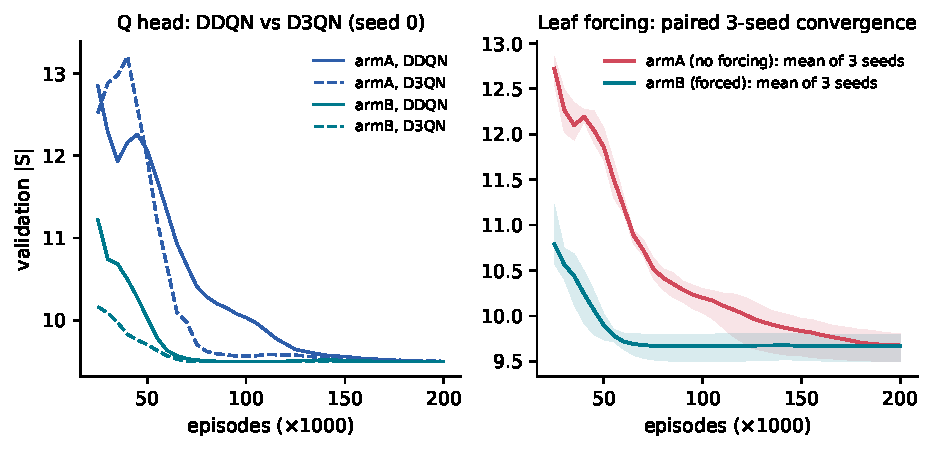
\includegraphics[width=0.95\textwidth]{figs/fig5_7_convergence.pdf}
  \caption{چپ: همگرایی \lr{DDQN} و \lr{D3QN} با seed یکسان. راست: اثر اجبار برگ
  روی میانگین سه seed با نوار کمینه–بیشینه.}
  \label{fig:convergence}
\end{figure}

حکم ما صریح است: \lr{D3QN} «بهتر نیست، ارزان‌تر است». ارزش آن صرفه‌جویی در
بودجه آموزش است، نه بهبود کیفیت پاسخ. همچنین باید توجه داشت که معیار
«اپیزود رسیدن به سطح فلات» یک معیار آستانه‌ای است؛ در یکی از seedها که مقدار
نهایی دقیقاً روی آستانه می‌نشیند، این معیار بی‌معنا می‌شود و عدد سرعت را نباید
به‌عنوان سرعت دیواری نقل کرد.

\section{دو تقویت صفر-آموزش}
\label{sec:boosts}

تا اینجا هر بهبود هزینه آموزش داشت. پرسش آخر این بود: از checkpointهای موجود،
بدون هیچ آموزش تازه، چقدر می‌توان گرفت؟ دو تقویت بررسی شد.

\subsection{پالایش خروجی (\lr{remove-redundant})}

چون \lr{TDSP} دقیقاً یک مسئله پوشش مجموعه‌ای است، پالایش کلاسیک روی \emph{هر}
جواب معتبر قابل اعمال است: اگر رأسی در $S$ باشد که همه همسایه‌هایش توسط
اعضای دیگر $S$ پوشش داده می‌شوند، حذف آن جواب را از احاطه‌گری کامل خارج
نمی‌کند.

\begin{lemma}
\label{lem:rr}
اگر $S$ احاطه‌گر کامل باشد و $v\in S$ حذف شود، مجموعه حاصل احاطه‌گر کامل
است به شرط آنکه هر $u\in N(v)$ عضوی از $S\setminus\{v\}$ داشته باشد. بنابراین
اندازه هرگز افزایش نمی‌یابد و خروجی همیشه شدنی می‌ماند.
\end{lemma}

\begin{proof}
برای هر $u\in N(v)$، همسایه‌ای در $S\setminus\{v\}$ موجود است (فرض لم). برای
سایر رأس‌ها، شاهدان پیشین دست‌نخورده‌اند چون تنها $v$ حذف شده و $v$ شاهد هیچ
رأسی جز همسایه‌هایش نبود.
\end{proof}

در پیاده‌سازی، این شرط نه فرض، بلکه \emph{خودِ آزمون} است: پس از هر حذف بررسی
می‌شود که مجموعه همچنان احاطه‌گر کامل است، و همچنین \lr{assert} می‌شود که اندازه
زیاد نشود. اثر عملی چشمگیر بود (شکل~\ref{fig:refinement}): روی گراف‌های متراکم،
\lr{armA} از $1.205$ به $1.059$ (حدود $12\%$ کوچک‌تر؛ در $55\%$ نمونه‌ها حداقل یک
رأس حذف شد) و \lr{paper-v2} از $1.310$ به $1.183$ بهبود یافت. روی گراف‌های اسپارس
اثر تقریباً صفر است، چون مجموعه‌های مدل از پیش کمینه‌اند.

\begin{figure}[ht]
  \centering
  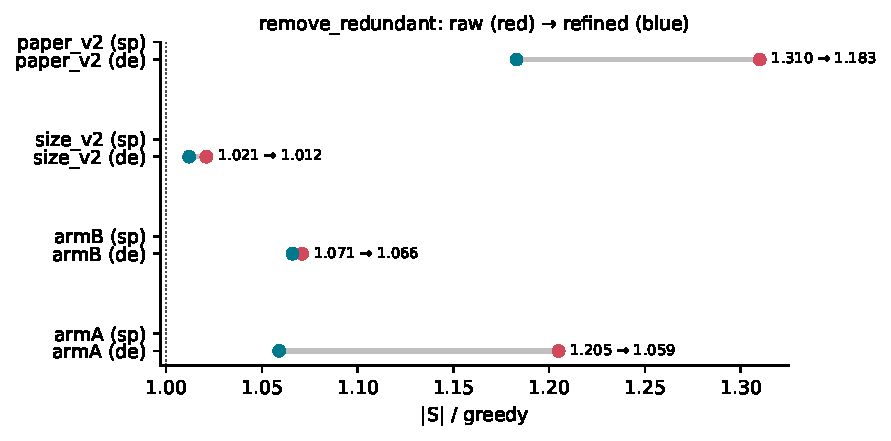
\includegraphics[width=0.62\textwidth]{figs/fig5_6_refinement.pdf}
  \caption{اثر \lr{remove-redundant} روی خروجی چهار \lr{checkpoint}.}
  \label{fig:refinement}
\end{figure}

همین پالایش یک ایراد روش‌شناختی در مقایسه‌های پیشین را آشکار کرد: در آزمایش
بازارزیابی، \lr{GRASP} \emph{درون خود} این پالایش را دارد، در حالی که مدل با
خروجی خام سنجیده می‌شد. پس از متقارن کردن این شرط، فاصله مدل و \lr{GRASP} به‌شدت
کم شد و ادعای «مدل به \lr{GRASP} می‌بازد» به «هم‌سطح» تغییر کرد.

\subsection{ماسک \lr{top-k} بر پایه سود}

در هر گام، به‌جای آنکه سیاست در میان همه رأس‌های مجاز انتخاب کند، فقط $k$ رأسِ
با بیشترین سود (تعداد همسایه‌های راضی‌نشده) قانونی اعلام می‌شوند و شبکه میان
آن‌ها انتخاب می‌کند. دو سر این طیف از پیش معلوم است: $k=1$ دقیقاً سیاست حریصانه
بومی است و $k=n$ همان سیاست آزاد. این تقویت، تعمیم عملی همان ایده «اولویت‌گذاری
نامزدها» است که در طرح اولیه دنبال می‌کردیم.

شکل~\ref{fig:topk} نتیجه جاروب را نشان می‌دهد: $k=3$ بهترین است
($1.205\rightarrow1.009$ برای \lr{armA}) و افزایش $k$ به $5$ و $10$ بدتر می‌شود.
تفسیر: سود از «حذف گزینه‌های کم‌سود» می‌آید، نه از آزادی بیشتر؛ یعنی سیاست در
گام‌هایی که یک رأس کم‌سود را ترجیح می‌دهد اشتباه می‌کند. ترکیب $k=3$ با پالایش
خروجی، مدل را به سطح \lr{GRASP} می‌رساند.

\begin{figure}[ht]
  \centering
  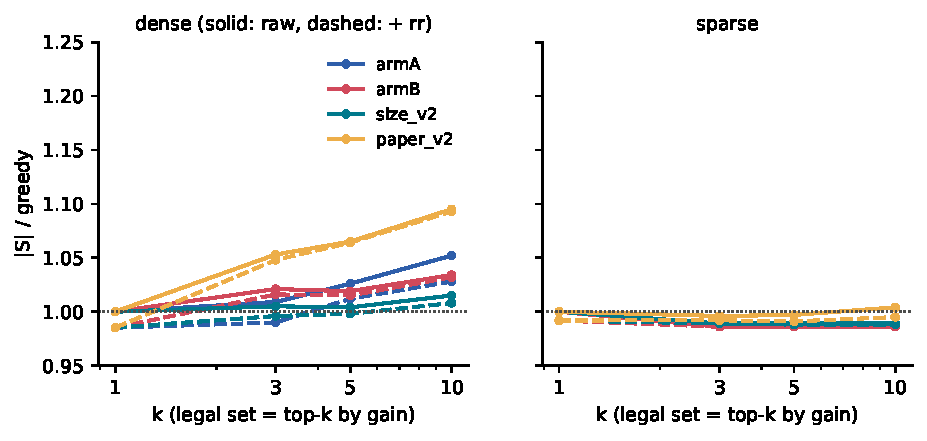
\includegraphics[width=0.95\textwidth]{figs/fig5_5_topk_sweep.pdf}
  \caption{جاروب ماسک \lr{top-k}: نسبت اندازه به حریصانه بر حسب $k$.}
  \label{fig:topk}
\end{figure}

برای آنکه ادعای «هوشمندی سیاست» با «کمک ماسک حریصانه» اشتباه نشود، دو کنترل
افزوده شد: (الف) \lr{greedy+rr}، یعنی همان پالایش روی سیاست بی‌هوش؛ (ب)
\lr{random@k+rr}، یعنی سکه‌انداختن در همان مجموعه $k$ رأسی. نتیجه
روی گراف‌های متراکم: \lr{armA@3+rr} برابر $0.990$، \lr{random@3+rr} برابر
$1.099$ و \lr{greedy+rr} برابر $0.995$؛ یعنی شبکه در همان مجموعه قانونی
$11$ واحد بهتر از سکه‌انداختن عمل می‌کند، ولی نسبت به حریصانه پالایش‌شده تقریباً
هم‌سطح است.

\section{ارزیابی جامع}
\label{sec:eval}

ارزیابی این فصل روی \num{168} نمونه گراف انجام شد: \num{88} گراف متراکم
(شبکه مستطیلی، شش‌گوش، مثلثی و \lr{ER/BA} تا $n=300$) و \num{80} گراف اسپارس
(درخت تصادفی و \lr{BA} با $m=1$ تا $n=200$)، با چهار \lr{checkpoint} و
\num{6888} مجموعه تولیدشده. همه مجموعه‌های تولیدشده یک‌بار دیگر به‌عنوان
احاطه‌گر کامل بررسی شدند: \emph{هیچ} خروجی ناشدنی وجود نداشت، هیچ‌گاه
\lr{remove-redundant} اندازه را افزایش نداد و ماسک با $k=1$ در \num{168} از
\num{168} نمونه دقیقاً همان جواب حریصانه بومی را داد (شاهد درست‌بودن پیاده‌سازی).

شکل~\ref{fig:quality} کیفیت را نسبت به حریصانه به تفکیک خانواده نشان می‌دهد و
جدول~\ref{tab:paired} نتیجه آزمون‌های زوجی را خلاصه می‌کند. آزمون‌ها روی گراف‌های
\emph{جفت‌شده} (یک شناسه برای هر گراف) انجام شده‌اند: بازه اطمینان بوت‌استرپ با
\num{10000} بازنمونه‌گیری و آزمون ویلکاکسون علامت‌دار.

\begin{table}[ht]
  \centering
  \caption{مقایسه‌های زوجی روی گراف‌های متراکم و اسپارس (معیار $|S|/|greedy|$)}
  \label{tab:paired}
  \begin{tabular}{lcccc}
    \toprule
    مقایسه & تفاوت میانگین & بازه اطمینان ۹۵٪ & $p$ & حکم \\
    \midrule
    \lr{armA@3+rr} در برابر \lr{greedy+rr} & $-0.0049$ & $[-0.019,\,+0.010]$ & $0.485$ & تساوی \\
    \lr{armA@3+rr} در برابر \lr{GRASP} & $+0.0026$ & $[-0.017,\,+0.023]$ & $0.851$ & تساوی \\
    \lr{armA@3+rr} در برابر \lr{random@3+rr} & $-0.109$ & $[-0.150,\,-0.071]$ & $1.5\times10^{-7}$ & شبکه مؤثر است \\
    \lr{armA} در برابر \lr{armA@3} & $+0.196$ & $[+0.155,\,+0.239]$ & $2\times10^{-11}$ & ماسک مؤثر است \\
    \lr{armA} در برابر \lr{armA+rr} & $+0.145$ & $[+0.110,\,+0.183]$ & $2\times10^{-9}$ & پالایش مؤثر است \\
    \lr{armB@3+rr} در برابر \lr{greedy+rr} & $+0.022$ & $[+0.004,\,+0.041]$ & $0.035$ & اندکی بدتر \\
    \lr{armA+F} در برابر \lr{GRASP} (اسپارس) & $+0.0001$ & $[0,\,+0.0004]$ & $0.317$ & تساوی \\
    \bottomrule
  \end{tabular}
\end{table}

\begin{figure}[ht]
  \centering
  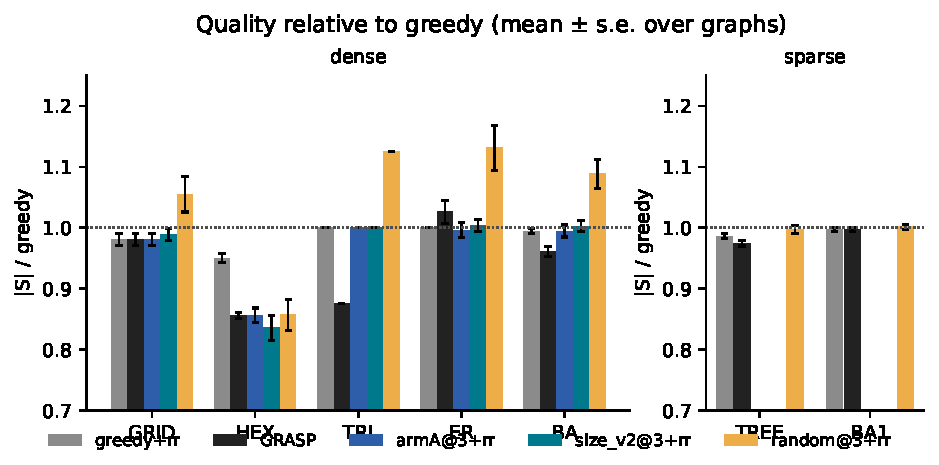
\includegraphics[width=0.98\textwidth]{figs/fig5_4_quality_by_family.pdf}
  \caption{کیفیت نسبت به حریصانه به تفکیک خانواده (میانگین $\pm$ خطای معیار).}
  \label{fig:quality}
\end{figure}

جمع‌بندی کمّی:

\begin{itemize}
  \item روی گراف‌های تصادفی متراکم، پیکربندی پیشنهادی
        (\lr{armA@3+rr}) با بازارزیابی \lr{GRASP} \emph{آماری} هم‌سطح است و
        از حریصانه پالایش‌شده هم بهتر نیست؛ برتری واقعیRL در این خانواده وجود
        ندارد و صادقانه گزارش می‌شود.
  \item روی گراف‌های اسپارس، مدل به بهینه می‌رسد
        ($|S|/\gamma_t=1.000$ برای هر دو بازوی آموزش‌دیده) و از
        \lr{greedy+rr} به‌طور آماری بهتر است ($p=4\times10^{-4}$)، هرچند
        اختلاف اندازه ناچیز است.
  \item روی لاتیس شش‌گوش، مدل \emph{واقعاً} برنده است: بهترین نتیجه فصل
        \lr{size-v2@3+rr} با نسبت $0.786$ در برابر \lr{GRASP} با $0.847$ و
        حریصانه پالایش‌شده با $0.959$ (شکل~\ref{fig:hex}).
  \item هزینه: مدل با تقویت‌ها روی گراف‌های متراکم حدود $0.015$ ثانیه و روی
        اسپارس $0.005$–$0.007$ ثانیه زمان می‌برد، در برابر $0.068$ ثانیه
        (\lr{GRASP} روی متراکم) و $0.163$ ثانیه (روی اسپارس)؛ یعنی حدود
        $4$ تا $25$ برابر سریع‌تر با کیفیت هم‌سطح (شکل~\ref{fig:timequality}).
\end{itemize}

\begin{figure}[ht]
  \centering
  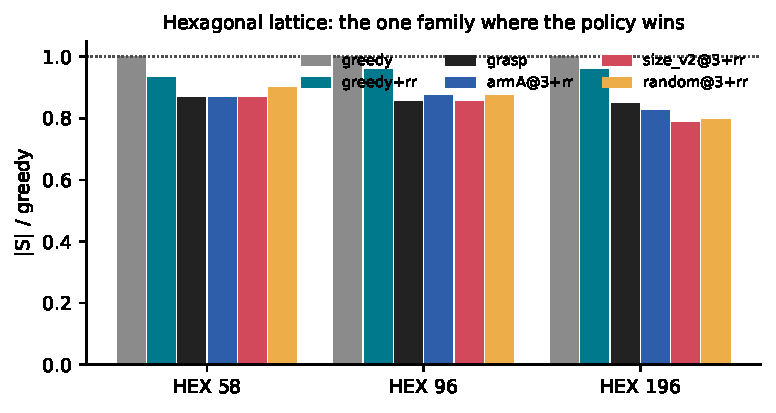
\includegraphics[width=0.72\textwidth]{figs/fig5_10_hex.pdf}
  \caption{خانواده شش‌گوش: تنها خانواده‌ای که سیاست به‌طور معنادار از
  بازارزیابی بهتر است.}
  \label{fig:hex}
\end{figure}

\begin{figure}[ht]
  \centering
  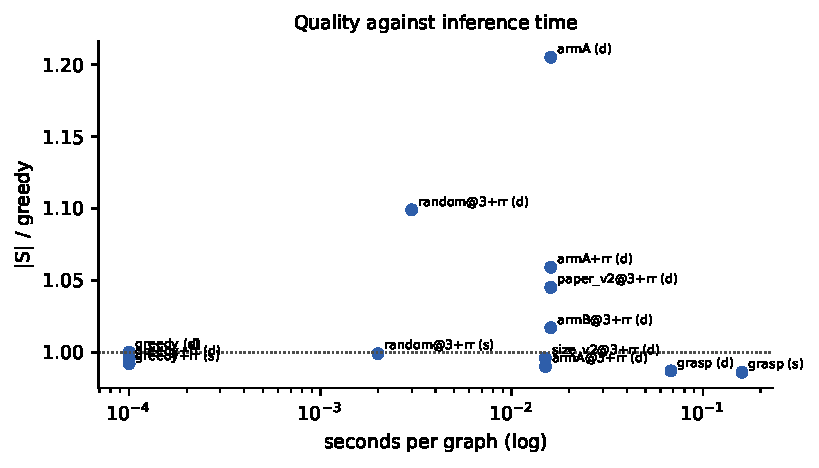
\includegraphics[width=0.72\textwidth]{figs/fig5_9_time_quality.pdf}
  \caption{کیفیت در برابر زمان استنتاج هر گراف (محور زمان لگاریتمی).}
  \label{fig:timequality}
\end{figure}

\section{مثال گام‌به‌گام: کل فرآیند روی یک گراف کوچک}
\label{sec:example}

برای اینکه خواننده بتواند همه اجزای بخش‌های پیشین را یک‌جا ببیند، فرآیند را روی
یک درخت تصادفی با $n=12$ رأس (seed پنجم) گام‌به‌گام اجرا می‌کنیم. برگ‌های این
درخت $\{1,2,3,4,11\}$ و مجموعه اجباری
$F=\{0,6,8,10\}$ است.

\textbf{گام صفر (اجبار).} $F$ در $S$ نشانده می‌شود. بنابراین $vf=1$ برای همه
همسایه‌های $F$، و برای خود اعضای $F$ مقدار $vf$ صفر می‌ماند، چون هنوز کسی
آن‌ها را احاطه نکرده است. این همان تفکیک دو کانال حالت
\eqref{eq:state} است: $ins$ برای اعضای $F$ یک و $vf$ صفر است.
شکل~\ref{fig:trace} (الف).

\textbf{گام یک (تصمیم شبکه).} نامزدهای قانونی همه رأس‌های خارج از $S$ هستند:
$\{1,2,3,4,5,7,9,11\}$. سود هر نامزد (تعداد همسایه‌های راضی‌نشده) محاسبه می‌شود؛
در این گام، رأس‌های $2,3,4$ بزرگ‌ترین سود ($1$) را دارند، پس با $k=3$ همان‌ها
قانونی می‌مانند. شبکه مقادیر $Q$ را برای نامزدهای قانونی محاسبه می‌کند و در
این نمونه:
\[
Q(2)=-3.732,\quad Q(3)=-3.767,\quad Q(4)=-3.767 .
\]
بیشینه، رأس $2$ است؛ پس عمل $a_1=2$، رأس $0$ راضی می‌شود
($vf_0:0\rightarrow1$) و پاداش $r=-1$ دریافت می‌شود (تعریف~\ref{def:size-reward}).
شکل~\ref{fig:trace} (ب).

\textbf{گام دو.} نامزدها اکنون $\{1,3,4,5,7,9,11\}$ هستند و سود بیشینه برای
$\{3,4,5\}$ برابر $1$ است. شبکه $Q(3)=-1.884$ را بیشینه می‌بیند و
$a_2=3$ انتخاب می‌شود؛ رأس $8$ راضی می‌شود و پاداش باز هم $-1$ است.

\textbf{پایان.} پس از این دو تصمیم، همه رأس‌ها $vf=1$ دارند و شرط پایان برقرار
است. مجموعه نهایی $S=\{0,2,3,6,8,10\}$ با اندازه $6$ است که با $\gamma_t=6$
(حل دقیق) برابر است. سیاست حریصانه بومی نیز همین اندازه را می‌دهد، اما
\lr{GRASP} و هر دو سیاست مدل روی این نمونه به بهینه رسیدند؛ نکته اصلی صرفه‌جویی
در تصمیم است: عامل فقط \emph{دو} تصمیم گرفت، در حالی که بدون $F$ باید شش تصمیم
می‌گرفت. شکل~\ref{fig:trace} (ج).

\textbf{حسابداری پاداش.} اگر پاداش سود به‌کار می‌رفت، مجموع آن در این اپیزود
دقیقاً $n=12$ می‌شد و هیچ ارتباطی با $|S|=6$ نداشت (قضیه~\ref{thm:gain}).
با پاداش هزینه، بازده تصمیم‌های عامل $-2$ است و با احتساب $|F|=4$ مجموعه‌ای،
بازده کل باز هم $-6=-|S|$ می‌شود؛ یعنی بازده دقیقاً همان تابع هدف است.

\begin{figure}[ht]
  \centering
  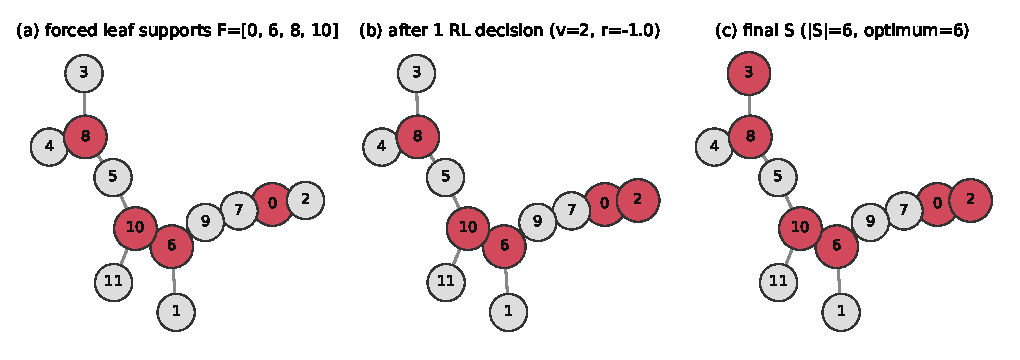
\includegraphics[width=0.98\textwidth]{figs/fig5_12_trace.pdf}
  \caption{اجرای گام‌به‌گام روی درخت $n=12$: (الف) نشاندن $F$؛ (ب) پس از یک تصمیم
  شبکه؛ (ج) مجموعه نهایی.}
  \label{fig:trace}
\end{figure}

\section{تهدیدهای اعتبار}
\label{sec:threats}

\begin{enumerate}
  \item \textbf{تعداد تکرار روی گراف‌های تصادفی:} برای \lr{ER} و \lr{BA} تنها
        \num{10} نمونه در هر اندازه تولید شده است (کمتر از آزمایش‌های فصل چهارم
        که \num{20} نمونه داشت). لتیس‌ها تک‌نمونه‌اند و نتیجه‌گیری قوی روی مثلثی
        مجاز نیست (تنها یک نمونه).
  \item \textbf{حل دقیق فقط تا $n\le120$:} بنابراین برای گراف‌های \lr{BA/ER}
        با $n=300$ و درخت‌ها با $n=200$، معیار $\gamma_t$ در دسترس نیست و مقایسه
        فقط با خط مبنای حریصانه انجام شده است.
  \item \textbf{تک‌seed بودن مدل‌های متراکم:} $size-v2$ و $paper-v2$ فقط با
        یک seed آموزش دیده‌اند؛ سه-seed فقط برای دو بازوی اسپارس انجام شده است.
        بنابراین ادعای «کیفیت» روی این دو \lr{checkpoint} به seed حساس است و در
        متن با همین قید نقل می‌شود.
  \item \textbf{معیار آستانه‌ای همگرایی:} عدد «$1.7$ برابر سریع‌تر» برای
        \lr{D3QN} بر پایه رسیدن به یک سطح آستانه تعریف شده و به انتخاب سطح فلات
        حساس است.
  \item \textbf{roll-out قطعی:} در ارزیابی، تصمیم‌گیری روی مقادیر $Q$ و بدون
        نمونه‌گیری انجام می‌شود؛ بنابراین نوسان تصادفی در نتایج آزمایش وجود ندارد
        و تنها منبع تصادفی، خودِ نمونه‌های گراف و کنترل \lr{random@k} است.
\end{enumerate}

% =============================================================================
%  فصل ششم — نتیجه‌گیری و پیشنهادها
% =============================================================================
\chapter{نتیجه‌گیری و پیشنهادها}
\label{ch:conclusion}

\section{خلاصه مسیر انجام پژوهش}
\label{sec:summary}

این پژوهش با بازسازی دقیق چارچوب \lr{Chen} و همکاران آغاز شد: شبکه عصبی
پیام‌رسان برای استخراج نمایش گراف، \lr{DDQN} برای تصمیم‌گیری متوالی، و یک
محیط پوشش‌محور که در هر گام یک رأس را انتخاب می‌کند. بازسازی انجام شد و نتایج
مقاله روی جدول‌های مرجع بازتولید گردید؛ اما بازسازی تنها نقطه شروع بود. مسیر
اصلی پژوهش سه مرحله داشت:

\begin{enumerate}
  \item \textbf{بررسی تعمیم‌پذیری چارچوب:} آیا اجزای روش مرجع را می‌توان به
        مسئله سخت‌گیرانه‌تر مجموعه احاطه‌گر کامل منتقل کرد؟
  \item \textbf{بهبود چارچوب برای مسئله هدف:} بازطراحی فضای عمل، بازتعریف تابع
        پاداش، رفع یک باگ مقیاس‌پذیری در معماری، و به‌کارگیری دانش نظریه گراف.
  \item \textbf{رقابت با روش‌های غیر‌یادگیری:} مقایسه با خط پایه حریصانه و
        بازارزیابی \lr{GRASP} با معیارهای کیفیت، شدنی‌بودن، زمان و همگرایی.
\end{enumerate}

\section{پاسخ به سؤالات تحقیق}
\label{sec:answers}

\begin{table}[ht]
  \centering
  \caption{پاسخ فشرده به سؤالات پژوهش و شاهد هر پاسخ}
  \label{tab:answers}
  \begin{tabular}{p{5.2cm}p{4.6cm}p{4.2cm}}
    \toprule
    سؤال & پاسخ & شاهد \\
    \midrule
    آیا بازتولید نتایج مقاله با دقت قابل قبول ممکن است؟
    & بله؛ تعریف جدول‌های مرجع بازتولید و انحراف‌ها ثبت شد
    & فصل چهارم و جداول مرجع \\
    آیا مفاهیم نظریه گراف فضای جست‌وجو را کاهش می‌دهند؟
    & بخشی: اجبار برگ‌ها تصمیم‌ها را حدود \num{64}\% کم می‌کند؛ اما قواعد
      کاهش کلاسیک در این دامنه فعال نمی‌شوند
    & بخش~\ref{sec:forcing}، جدول~\ref{tab:forcing} \\
    آیا می‌توان فرآیند یادگیری را بهبود داد؟
    & بله؛ اجبار برگ‌ها همگرایی را حدود \num{3.5} برابر سریع‌تر و سر دوگانه آن
      را حدود \num{1.7} برابر سریع‌تر می‌کند
    & شکل~\ref{fig:convergence} \\
    آیا کیفیت پاسخ رقابتی است؟
    & هم‌سطح با \lr{GRASP} با اختلاف آماری ناچیز، و برتری معنادار روی لاتیس
      شش‌گوش؛ اما روی \lr{BA} بازنده
    & جدول~\ref{tab:paired}، شکل~\ref{fig:hex} \\
    آیا چارچوب به \lr{TDSP} تعمیم‌پذیر است؟
    & بله؛ اما نه با ماسک مقاله؛ نیازمند بازطراحی فضای عمل (قضیه~\ref{thm:mask})
    & بخش~\ref{sec:mask}، شکل~\ref{fig:actionspace} \\
    وضعیت زمان اجرا چگونه است؟
    & \num{4} تا \num{25} برابر سریع‌تر از \lr{GRASP} با کیفیت هم‌سطح
    & شکل~\ref{fig:timequality} \\
    \bottomrule
  \end{tabular}
\end{table}

\section{مشارکت‌های پژوهش}
\label{sec:contributions}

\begin{enumerate}
  \item \textbf{قضیه ناسازگاری ماسک و نمونه نقض کمینه:} نشان داده شد که ماسک
        عمل چارچوب مرجع، ذاتاً (و نه به‌دلیل ضعف آموزش) ناتوان از تولید جواب
        برای \lr{TDSP} است؛ این نتیجه با اثبات ریاضی، با \num{177} آزمایش
        محاسباتی و با مثال نقض $P_4$ پشتیبانی می‌شود.
  \item \textbf{محیط بازطراحی‌شده با حالت دوکاناله:} قاعده گذار جدید (انتخاب
        $v$ تنها $N(v)$ را راضی می‌کند) به‌همراه حالت $[vf,ins]$ و پاداش هزینه،
        مسئله را بدون تغییر در حلقه یادگیری و شبکه قابل حل کرد.
  \item \textbf{اصلاح باگ مقیاس‌پذیری خوانش گراف:} تشخیص اینکه جمع‌کردن
        نمایش رأس‌ها باعث انفجار مقادیر $Q$ با $n$ می‌شود، و اصلاح آن با تجمیع
        میانگین؛ این اصلاح کیفیت روی گراف‌های بزرگ را از $4.34$ به $1.04$
        رساند.
  \item \textbf{اجبار برگ‌ها به‌جای حذف آن‌ها:} تبدیل یک قاعده کاهش نامعتبر
        (که با مثال $P_3$ رد می‌شود) به یک راهبرد معتبر و مؤثر، با اثبات درستی
        و اندازه‌گیری اثر روی کیفیت و همگرایی.
  \item \textbf{دو تقویت صفر-آموزش:} پالایش خروجی مبتنی بر مشاهده هم‌ارزی
        \lr{TDSP} با مسئله پوشش مجموعه‌ای، و ماسک \lr{top-k} سودمحور، هر دو
        بدون هیچ آموزش تازه و با اثبات حفظ شدنی‌بودن.
  \item \textbf{پروتکل ارزیابی چند-seed و زوجی:} تکرار آموزش با سه seed و
        مقایسه زوجی (همان seed، دو پیکربندی) که نشان داد اثر اجبار نقطه پایان
        را تغییر نمی‌دهد و تنها سرعت رسیدن به آن را عوض می‌کند.
\end{enumerate}

\section{قلمرو روش: کجا مفید است و کجا نیست}
\label{sec:scope}

جمع‌بندی نتایج، تصویر دقیقی از جایگاه روش ارائه می‌دهد که برای استفاده عملی
ضروری است:

\begin{itemize}
  \item \textbf{برنده:} لاتیس شش‌گوش و خانواده‌های اسپارس (درخت، \lr{BA} با
        $m=1$). روی شش‌گوش، مدل با تقویت‌ها از \lr{GRASP} بهتر است
        ($0.786$ در برابر $0.847$) و روی اسپارس کیفیت بهینه است.
  \item \textbf{هم‌سطح:} شبکه مستطیلی، مثلثی و \lr{ER}؛ اینجا مسئله اشباع شده و
        فاصله معناداری میان روش‌ها وجود ندارد.
  \item \textbf{بازنده:} گراف‌های \lr{BA} متراکم، که \lr{GRASP} در آن‌ها بهتر
        است. دستیابی به برتری در این خانواده نیازمند آموزش چند‌اندازه و بودجه
        محاسباتی بیشتر است.
  \item \textbf{مزیت پایدار روش:} زمان استنتاج ثابت و کوچک. مدل یک بار آموزش
        می‌بیند و سپس با یک گذر شبکه‌ای جواب می‌دهد؛ این ویژگی در کاربردهای
        بی‌درنگ (شبکه حسگر، تخصیص منابع) که مسئله باید مکرر و سریع حل شود،
        ارزش عملی دارد.
\end{itemize}

\section{محدودیت‌ها}
\label{sec:limits}

محدودیت‌های اصلی همان‌هایی است که در بخش~\ref{sec:threats} فهرست شد: تعداد
محدود تکرار روی گراف‌های تصادفی، در دسترس نبودن حل دقیق برای $n>120$، آموزش
تک‌seed برای دو \lr{checkpoint} متراکم، حساسیت معیار همگرایی به سطح آستانه و
قطعی بودن \lr{roll-out} در ارزیابی. افزون بر این‌ها، سه محدودیت روش‌شناختی را
باید صریح اعلام کرد:

\begin{enumerate}
  \item بخشی از آزمایش‌ها روی سخت‌افزار متفاوت (واحد پردازش گرافیکی و پردازنده
        مرکزی) اجرا شده است. پروتکل و seed یکسان بوده، اما دنباله اعداد تصادفی
        در این دو محیط یکی نیست؛ بنابراین آن دو اجرا کپی بیتی یکدیگر نیستند و
        مقایسه در سطح پروتکل انجام شده است.
  \item گزارش مقاله مرجع برای هر اندازه گراف یک مدل جداگانه آموزش می‌دهد؛
        در این پژوهش نیز برای هم‌خوانی همان رویه دنبال شد، اما در آزمایش‌های
        اسپارس یک مدل واحد روی چند اندازه آزمون شد که طبیعتاً سخت‌گیرانه‌تر است.
  \item ادعاهای کیفیت روی گراف‌های تصادفی به میانگین نمونه محدود است؛ در
        لتیس‌ها اندازه نمونه کوچک است و نتایج آن‌ها را نباید تعمیم داد.
\end{enumerate}

\section{پیشنهادهای کارهای آینده}
\label{sec:future}

\begin{enumerate}
  \item \textbf{الگوریتم‌های جایگزین:} ارزیابی روش‌های روی‌سیاستی مانند
        \lr{PPO} که با حذف \lr{replay buffer} تعریف حافظه مقاله را زیر سؤال
        می‌برند، و شبکه‌های گرافی قوی‌تر مانند \lr{GIN} برای مقایسه دقیق‌تر
        توان نمایش.
  \item \textbf{آموزش چند‌اندازه:} تعلیم یک مدل روی ترکیبی از اندازه‌ها و
        خانواده‌ها، برای آزمون برتری روی \lr{BA} و گراف‌های بزرگ‌تر؛ این مسیر
        در فضای \lr{CPU} گران است و اجرای موازی یا استفاده از شتاب‌دهنده
        توصیه می‌شود.
  \item \textbf{ترکیب یادگیری و جست‌وجو:} به‌کارگیری خروجی شبکه به‌عنوان جواب
        اولیه برای جست‌وجوی محلی یا برنامه‌ریزی محدود (\lr{look-ahead})؛ چون
        خروجی مدل از پیش شدنی است، بهبودهای جزئی روی آن ارزان هستند.
  \item \textbf{تعمیم به اهداف ترکیبی:} نسخه‌های وزن‌دار (\lr{$k$-domination})
        یا احاطه‌گری با محدودیت بودجه، که در آن‌ها یک چارچوب یادگیری‌محور با
        سرعت استنتاج ثابت مزیت بیشتری نشان می‌دهد.
  \item \textbf{ارزیابی احتمال‌محور:} گزارش بازه اطمینان روی همه ادعاهای کیفیت
        و افزودن seedهای بیشتر برای مدل‌های متراکم، تا نتایج در برابر انتخاب
        تصادفی مقاوم شوند.
  \item \textbf{مطالعه اثر معماری سر شبکه:} بررسی اینکه آیا ترکیب ماسک
        \lr{top-k} با سرهای پیشرفته‌تر (مثل سر مزیت تفکیک‌شده چند‌لایه) می‌تواند
        آن $11$ واحد فاصله با سیاست تصادفی را در خانواده‌های متراکم نیز به
        برتری نسبت به خط مبنا تبدیل کند.
\end{enumerate}


% ------------------------------------------------------------------- منابع
\chapter*{منابع}
\addcontentsline{toc}{chapter}{منابع}
\begin{latin}
\bibliographystyle{unsrt}
\bibliography{refs}
\end{latin}

% ------------------------------------------------------------------- واژه‌نامه
\chapter*{واژه‌نامه فارسی به انگلیسی}
\addcontentsline{toc}{chapter}{واژه‌نامه فارسی به انگلیسی}
\begin{latin}
\begin{center}
\begin{tabular}{ll}
\toprule
Persian & English \\
\midrule
مجموعه احاطه‌گر & Dominating Set \\
مجموعه احاطه‌گر کامل & Total Dominating Set \\
شبکه عصبی گرافی & Graph Neural Network \\
شبکه عصبی پیام‌رسان & Message Passing Neural Network \\
یادگیری تقویتی & Reinforcement Learning \\
حافظه بازپخش & Experience Replay Buffer \\
بازارزیابی حریصانه تصادفی & GRASP \\
سر دوگانه & Dueling Head \\
پوشش مجموعه‌ای & Set Cover \\
\bottomrule
\end{tabular}
\end{center}
\end{latin}

\end{document}
